%
% Draft  document solvedme.tex
% Notes on solving the dyadic model equations
%
 
\documentclass[titlepage]{article}  % Latex2e
\usepackage{graphicx,lscape,subfigure}
\usepackage{bm}
\usepackage{textcomp}
 

\title{ Solving the Dyadic Model Equations}
\author{Neville Jackson }
\date{18 May 2015 \\
      For dmm\_1.6-2}   % Deleting this command produces today's date.

 
\begin{document} 
 
\maketitle      
\tableofcontents

\section{Introduction} 
The function {\em dmm()} sets up equations which relate the observed covariance of pairs of individuals or dyads, to their expectation in terms of postulated genetic and environmental variance and covariance components.

These equations, termed dyadic model equations (DME's), can be solved directly to obtain estimates of variance and covariance components.  The DME's are linear equations, and are exactly analogous to a set of multi-trait multiple regression equations. 

The function {\em dmm()} therefore effectively turns variance component estimation into a regression problem. All of the statistical techniques for fitting a linear multiple regression are therefore available for solving the DME's. The function {\em dmm()} uses the QR algorithm by default, but can optionally use {\em lm()}, robust regression ({\em lmrob()}), or principal component regression ({\em pls package}).

This document is about the practical issues in checking out a particular set of DME's and in choosing an appropriate regression method for their solution.  In many of the datasets available to quantitative geneticists, the (co)variance components which we would like to estimate are partially confounded, sometimes to the point where they  are not separably estimable. This is particularly so in dealing with nonadditive genetic components. The function {\em dmm()} offers an experimental approach which allows partially confounded components to be estimated by constraining some components, using principal component regression.
 
\section{The dyadic model equations}
The dyadic model is presented in Section 6.2.2  of the document {\em dmmOvervire.pdf}~\cite{jack:15}. It results in a set of equations (the DME's) which are given in matrix form as equation 12, which is reproduced below

\begin{equation}
\mbox{\boldmath $\Psi = W \Gamma + \Delta$}   \label{eq.dme}
\end{equation}

It is important to understand each of the matrix components of these equations, so we elaborate as follows

First, the following variables set the size of the problem and the sizes of the above matrices
\begin{description}
\item[n] number of individuals with data
\item[m] number of individuals in pedigree
\item[l] number of traits
\item[k] number of fixed effects
\item[c] number of variance components to be estimated
\end{description}

Now we explain each matrix 
\begin{description}
\item[$\bm{\Psi}$] $n^{2} \times l^{2}$ matrix of dyadic covariances for each pair of individuals (row) and each traitpair (col). Each covariance needs to be appropriately adjusted for fixed effects. The columns of $\bm{\Psi}$ become the dependent variables in a multi-trait multiple regression.
\item[$\bm{W}$] $n^{2} \times c$ matrix containing the coefficients of the dyadic model equations, which become the independent variables of a multiple regression. Each column of $\bm{W}$ has the form $Vec{\bm{(MZ_{c} R_{c} Z_{c}^{\prime}M^{\prime})}}$ where $Vec$ is an operator that vectorizes a matrix, $\bm{M}$ is a matrix from the fixed effect model such that \mbox{\boldmath $Y - X \hat{\alpha} = M Y$}, $\bm{Z_{c}}$ is an incidence matrix relating individuals with data to individuals in the pedigree, and $\bm{R_{c}}$ is a relationship matrix relevant to component $c$. Note that relationship matrices are used, not their inverse.
\item[$\bm{\Gamma}$] $c \times l^{2}$ matrix of (co)variance component parameters to be estimated, which become the partial regression coefficients of a multiple regression.
\item[$\bm{\Delta}$] $n^{2} \times l^{2}$ matrix of dyadic model residuals. Note the variance of these is not the individual environmental variance component - that has to be explicitely fitted as one of the columns of matrix $\bm{W}$ and appears as one row of matrix $\bm{\Gamma}$. The $\bm{\Delta}$ matrix elements are the extent to which each dyadic covariance in matrix $\bm{\Psi}$ deviates from its expectation. The (co)variances of the elements of $\bm{\Delta}$ enter into the standard errors of variance component estimates, in the same way that the (co)variances of residuals enter into the standard errors of any regression coefficient estimates. 
\end{description}

Matrices $\bm{\Psi}$ and $\bm{W}$ have $n^{2}$ rows, so we are looking at solving $n^{2}$ equations in $c$ unknowns. This is an overdetermined system. We can use least squares to obtain an approximate solution. 

\section{Checking the dyadic model assumptions}
Before attempting a regression fit of model (1), it is worth looking at how well the data conform to the assumptions made in using using least squares to fit a multiple regression model. The critical assumptions are

\begin{itemize}
\item the independent variables ( columns of $\bm{W}$) are uncorrelated
\item the residuals (columns of $\bm{\Delta}$) are uncorrelated with each other and with the independent variates
\end{itemize}

A least squares fit does not involve assumptions regarding the distribution of residuals, but this does become involved when using residuals to obtain standard errors of parameter estimates.

\subsection{The assumption of independence of columns of $\bm{W}$}

The correlations among independent variables (columns of $\bm{W}$) are returned by {\em dmm()} in the attribute {\em dme.correl} of the returned object.  These are pairwise correlations between the columns of the $\bm{W}$ matrix. They are not quite the same thing as correlations between relationship matrix elements, because the columns of $\bm{W}$ also involve $\bm{M}$ and $\bm{Z}$ matrices.

The $\bm{Z}$ matrix simply selects a subset of the relationship matrix corresponding to those individuals which have observations. The $\bm{M}$ matrix comes from the fixed effects model, and consists of a set of weights which adjust for the degrees of freedom involved in each of the fixed effects applicable to each individual. So the columns of the $\bm{W}$ matrix are a weighted subset of the elements of the appropriate relationship matrix. Their correlations are therefore not the same as relationship matrix element correlations.

In the case of a dataset with mean only, and all individuals in the pedigree with data, such as the {\em warcolak} dataset, the subset is all of the relationship matrix and the weights in $\bm{M}$ are all equal, so the correlations of the columns of $\bm{W}$ are exactly the same as the correlations of the elements of the relationship matrices, in this special case.

In regression analysis it is generally considered that if there are collinearities among the independent variates amounting to correlations greater than around 0.5 then the estimates of regression coefficients are suspect. Translating this to our dyadic model, the variance component estimates are not likely to achieve a realistic separation if the columns of $\bm{W}$ have correlations exceeding 0.5. The option of using principal component regression ({\em dmeopt="pcr"} has been developed as an experimental approach to dealing with serious collinearities among the components.

If we want to plot these correlations ( eg as scatteplots) we need argument {\em dmekeep=T} in calling {\em dmm()}. The dafault for {\em dmm()} is not to save the DME's in its return object. This can be overridden with argument {\em dmekeep=T}. This results in 2 attributes {\em dme.psi} and {\em dme.wmat} being added to the returned object. Caution, this can result in a very large returned object. The attribute {\em dme.wmat} is the $\bm{W}$ matrix, and its columns can be plotted with the standard {\em plot()} routine.

\subsection{The assumptions of independence of dyadic residuals}
To check the dyadic residuals, we can use the S3 {\em plot()} method included in the {\em dmm} package. This will output histograms, qqnorm plots, and scatterplots of residuals against fitted and observed values. Plots tend to be more informative for datasets with smaller numbers of individuals.

Dyadic residuals are usually not far from normally distributed, but may be leptokurtic and slightly skewed to the right.

If dyadic residuals are correlated with fitted values of the components, then there is something wrong with the model, probably some extra component should be fitted. 

One can expect dyadic residuals to be correlated with observed dyadic covariances. It is normal for the fitted components in a dyadic model to explain only a small fraction of the total variation, and this of course leads to the observed covariances being highly correlated with residuals.

The question of patterns of correlation among the dyadic residuals themselves is a seriously difficult area. The covariances (or correlations) among the dyadic residuals for one trait form an $n^{2} \times n^{2}$ matrix - ie $n^{4}$ elements. Too many to compute and cant be stored in R. This issue is discussed in the document {\em dmmOverview.pdf}~\cite{jack:15} in relation to why {\em dmm()} is not able to do REML estimates. REML estimates require that the covariance (or correlation) matrix of the dyadic residuals be constructed and used to compute a GLS rather than an OLS solution to the DME's. That is not computationally feasible, and neither is an examination of the residual covariance/correlation matrix.

The covariance structure of dyadic residuals is actually known. It is derived in Searle et al (1992)~\cite{sear:92} on pages 407-413. It involves fourth moments of the observations.

\section{An example using the {\em warcolak} dataset}
Using the {\em warcolak} dataset from the {\em nadiv} package (Wolak(2014)~\cite{wola:14}, and just analysing Trait2, we first setup the data file making all the appropriate relationship matrices, then run the usual analysis fitting 4 variance components,  using the default "qr" option for solving the DME's, and setting options to save the DME's and the fit object.

\begin{verbatim}
> library(dmm)
> data(warcolak)
> warcolak.df <- warcolak.convert(warcolak)
> warcolak.mdf.univ <- mdf(warcolak.df,pedcols=c(1:3),factorcols=4,ycols=c(5:6),
               sexcode=c(0,1),relmat=c("E","A","D","S"),keep=T)
  .....
> warcolak.fit.t2 <- dmm(warcolak.mdf.univ, Trait2 ~ 1,
            components=c("VarE(I)","VarG(Ia)", "VarG(Id)","VarGs(Ia)"),
            relmat = "withdf",dmekeep=T,dmekeepfit=T)
  .....
> summary(warcolak.fit.t2)
  .....
Components partitioned by DME from residual var/covariance after OLS-b fit:

              Traitpair Estimate StdErr CI95lo CI95hi
VarE(I)   Trait2:Trait2    0.270 0.0369  0.198  0.342
VarG(Ia)  Trait2:Trait2    0.313 0.0134  0.287  0.339
VarG(Id)  Trait2:Trait2    0.327 0.0380  0.252  0.401
VarGs(Ia) Trait2:Trait2    0.146 0.0130  0.121  0.172
VarP(I)   Trait2:Trait2    1.056 0.0142  1.028  1.084

\end{verbatim}

These results are as for Trait 2 in the bivariate analysis reported in dmmOverview.pdf~\cite{jack:15}. The only difference is that we have samed some additional information. 

The correlations among columns of $\bm{W}$ are, of course, also the same

\begin{verbatim}
> warcolak.fit.t2$dme.correl
            VarE(I)  VarG(Ia)  VarG(Id) VarGs(Ia)
VarE(I)   1.0000000 0.4856317 0.9190589 0.4081477
VarG(Ia)  0.4856317 1.0000000 0.6255694 0.8266557
VarG(Id)  0.9190589 0.6255694 1.0000000 0.5254541
VarGs(Ia) 0.4081477 0.8266557 0.5254541 1.0000000
>
\end{verbatim}

Two of these correlations are somewhat larger than the nominal 0.5 mentioned above. We need to look and see if the multiple regression has been able to separate these 4 components properly. To that end we will redo the analysis using {\em dmeopt="pcr"} instead of the default {\em "qr"}. Using the principal component regression option requires at least two runs - the first retaining all 4 principal components, and then one or more reruns omitting the least important principal components. The first run is as follows

\begin{verbatim}
> warcolak.fitpcr1 <- dmm(warcolak.mdf.univ, Trait2 ~ 1,
            components=c("VarE(I)","VarG(Ia)","VarG(Id)","VarGs(Ia)"),
            relmat = "withdf",dmekeep=T,dmekeepfit=T,dmeopt="pcr")
  .....
DME substep:
PCR option on dyadic model equations:
Data: 	X dimension: 29160000 4 
	Y dimension: 29160000 1
Fit method: svdpc
Number of components considered: 4

VALIDATION: RMSEP
Cross-validated using 10 random segments.
       (Intercept)  1 comps  2 comps  3 comps  4 comps
CV           1.023    1.022    1.022    1.022    1.022
adjCV        1.023    1.022    1.022    1.022    1.022

TRAINING: % variance explained
       1 comps   2 comps   3 comps    4 comps
X     79.46086  92.89539  99.28012  100.00000
evec   0.02946   0.03157   0.03158    0.03158
DME substep completed:
OLS-b step completed:
> 
> loadings(warcolak.fitpcr1$dme.fit)
Loadings:
            Comp 1 Comp 2 Comp 3 Comp 4
`VarE(I)`    0.209  0.663  0.192 -0.692
`VarG(Ia)`   0.699        -0.705       
`VarG(Id)`   0.275  0.630  0.111  0.718
`VarGs(Ia)`  0.626 -0.393  0.674       

               Comp 1 Comp 2 Comp 3 Comp 4
SS loadings      1.00   1.00   1.00   1.00
Proportion Var   0.25   0.25   0.25   0.25
Cumulative Var   0.25   0.50   0.75   1.00
>
\end{verbatim}

What we need from this at the moment is the \% of variance explained by various numbers of principal components. Obviously using all 4 components explains 100\% of the variation, but what is interesting is that  3 components explain 99\% and 2 components 92\%. This is a signal that we should try regressing the observations on 3 principal components of the columns of $\bm{W}$, and see how it affects the estimates and their standard errors. We do that with a rerun

\begin{verbatim}
> warcolak.fitpcr2 <- dmm(warcolak.mdf.univ, Trait2 ~ 1,
            components=c("VarE(I)","VarG(Ia)","VarG(Id)","VarGs(Ia)"),
            relmat = "withdf",dmeopt="pcr",ncomp=3)
  .....

> summary(warcolak.fitpcr2)
Call:
summary.dmm(object = warcolak.fitpcr2)

Coefficients fitted by OLS for fixed effects:

   Trait Estimate StdErr CI95lo CI95hi
1 Trait2   -0.063 0.0138  -0.09 -0.036


Components partitioned by DME from residual var/covariance after OLS-b fit:

              Traitpair Estimate StdErr CI95lo CI95hi
VarE(I)   Trait2:Trait2    0.286 0.0127  0.262  0.311
VarG(Ia)  Trait2:Trait2    0.315 0.0182  0.279  0.351
VarG(Id)  Trait2:Trait2    0.310 0.0118  0.286  0.333
VarGs(Ia) Trait2:Trait2    0.146 0.0205  0.106  0.186
VarP(I)   Trait2:Trait2    1.057 0.0244  1.010  1.105

> 
\end{verbatim}

So comparing these estimates with those from the "qr" fit (which are the same as obtained with "pcr" with all 4 principal components), we find that omitting one principal component has not changed the estimated components substantially, and has reduced the standard errors of the two constrained components.  By omitting the fourth principal component we have in effect set it to zero, which amounts to constraining the components estimates to be on the plane defined by

\begin{equation}
  -0.692 \times VarE(I) + 0.718 \times VarG(Id) = 0
\end{equation}

We get this equation from the {\em loadings} which were given at the end of the run with all four principal components above. If we substitute the estimates of VarE(I) and VarG(Id) from the 3 component run into the above equation we find that they do indeed fall on the constraint plane. So we still get estimates of all 4 components, but two of them are constrained to be in a ratio $0.692/0.718$, or approximately equal. 

To my mind, that is a more satisfactory analysis than the unconstrained result from  a"qr" fit. By regressing on the principal components of columns of $\bm{W}$ instead of on the columns themselves we have avoided violating the assumption of independence, and by applying one constraint we have improved the standard errors.

One can go on and try omitting two principal components. This leads to two constraint equations, so the variance components would be constrained to lie on the intersection of two planes. We shall not do it here. We have done enough to demonstrate the method. 

We can view the dyadic residuals using the S3 {\em plot()} method included in the {\em dmm} package. We do this for the "qr" fit as follows

\begin{verbatim}
> postscript(onefile=F,horizontal=F)
> plot(warcolak.fit.t2)
  .....
> dev.off()
\end{verbatim}

Five plots will be saved on five separate files. It is probably better to use {\em png()} rather than {\em postscript()}. The resulting plots are shown in Figure 1 to Figure 5. We can see that the histogram is more peaked than a normal distribution (Figure 1), that the qqplot is sigmoidal (Figure 2), that the residuals are not associated with fitted values ( Figure 3), that the observed values are strongly correlated with the residuals (Figure 4), and that the fitted values and observed values are not strongly correlated (Figure 5). There is some discussion of these aspects in the next section.

%\documentclass{article}
%\usepackage{graphicx,subfigure}
%\begin{document}

\begin{figure}[h]
  \centering
  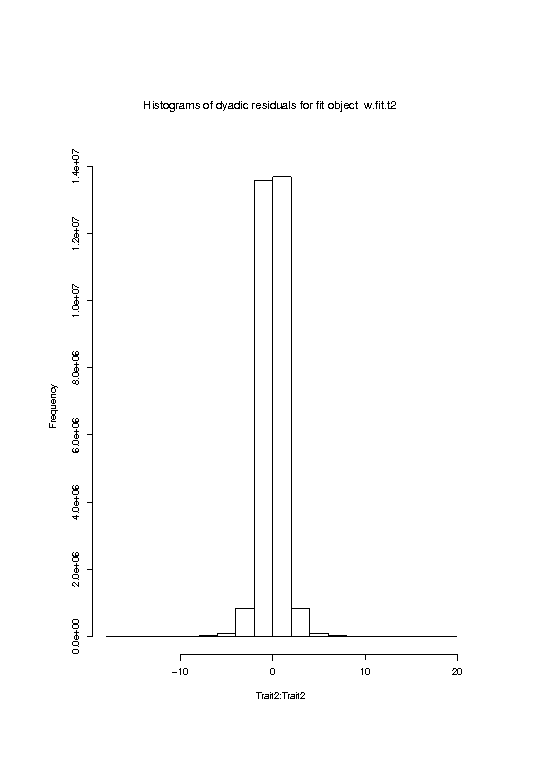
\includegraphics[width=1.1\textwidth]{Rplot001.png}
  \caption{Histogram of dyadic residuals for Trait2 of warcolak dataset
           with four components fitted usng "qr" method}
  \label{fig:1}
\end{figure}

%\end{document}


%\documentclass{article}
%\usepackage{graphicx,subfigure}
%\begin{document}

\begin{figure}[h]
  \centering
  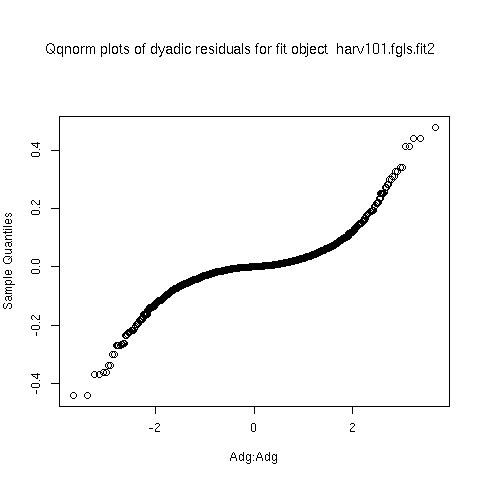
\includegraphics[width=0.5\textwidth]{harv101fig2.png}
  \caption{A qqplot of dyadic residuals for the Harvey dataset
           with two components fitted usng "fgls" method}
  \label{fig:2}
\end{figure}

%\end{document}


%\documentclass{article}
%\usepackage{graphicx,subfigure}
%\begin{document}

\begin{figure}[h]
  \centering
  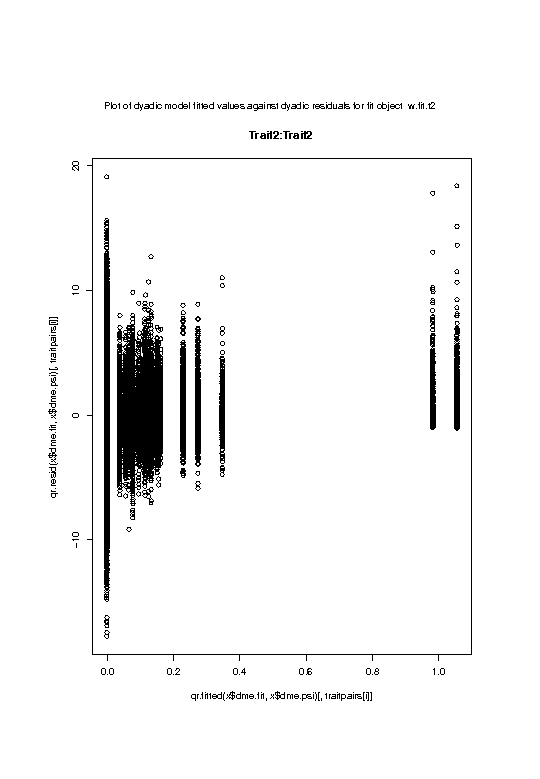
\includegraphics[width=1.1\textwidth]{Rplot003.png}
  \caption{A plot of dyadic model fitted values against dyadic residuals
     for Trait2 of warcolak dataset with four components fitted usng "qr" method}
  \label{fig:3}
\end{figure}

%\end{document}


%\documentclass{article}
%\usepackage{graphicx,subfigure}
%\begin{document}

\begin{figure}[h]
  \centering
  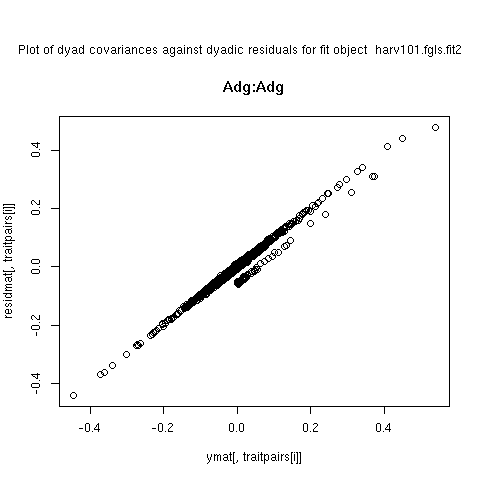
\includegraphics[width=0.5\textwidth]{harv101fig4.png}
  \caption{A plot of dyadic model observed values ( ie covariances)  against dyadic residuals
     for Trait  ADG of Harvey dataset with two components fitted usng "fgls" method}
  \label{fig:4}
\end{figure}

%\end{document}


%\documentclass{article}
%\usepackage{graphicx,subfigure}
%\begin{document}

\begin{figure}[h]
  \centering
  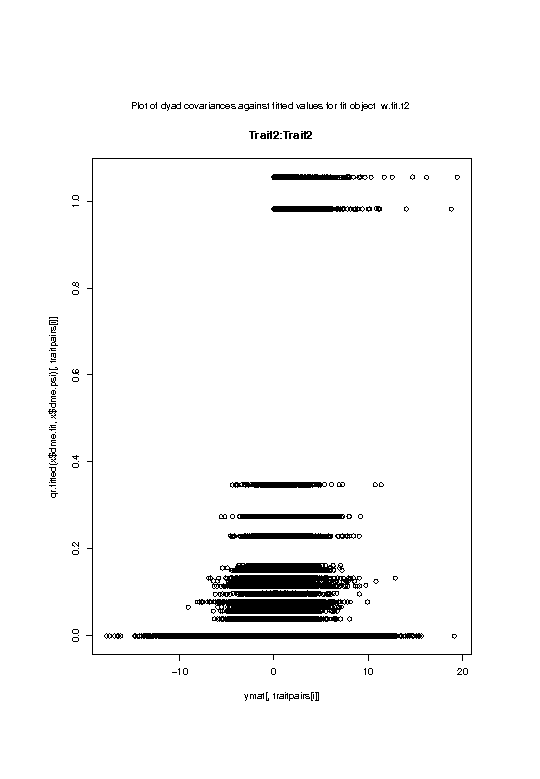
\includegraphics[width=1.1\textwidth]{Rplot005.png}
  \caption{A plot of dyadic model observed values against dyadic model fitted values
     for Trait2 of warcolak dataset with four components fitted usng "qr" method}
  \label{fig:5}
\end{figure}

%\end{document}



\section{Discussion}
There is nothing special about the dyadic model used by {\em dmm()}. Quantitative genetics has always been about covariances between relatives and measures of relationship, that is about pairs of individuals. It is just not usually called a dyadic model, but that is what it is. The term is common in the social sciences where interactions between pairs of individuals  are analysed with a dyadic model.

What is important is what the dyadic model allows us to do, not the terminology. By turning variance component estimation into a regression problem, a dyadic model opens the door to using the wide range of established regression techniques for variance component estimation. That includes techniques for dealing with collinearities among the independent variables, and these could be quite useful in quantitative genetic applications where the variance components which we wish to estimate are often partially confounded, as in the example above. There is a full presentation on the use of principal components regression in {\em dmmOverview.pdf}~\cite{jack:15} Section 7.4. There are some issues, the interface to the "pcr" option via the {\em pls} package is clumsy and its use is seriously memory intensive. Some further work is indicated.

The dyadic residuals ($\bm{\Delta}$) are usually large and highly correlated with the observed dyadic covariances ($\bm{\Psi}$), as in Figure 4. This is because the covariance for each dyad is obtained from only one replicate pair of observations. The $R^{2}$ for a dyadic model is tiny - only 3 percent of the variance in the case of the {\em warcolak} example above. This highlights the central problem of quantitative genetic analysis - it is trying to extract information from a system with a signal to noise ration of $0.03$. Modelling variances is much more demanding than modelling observations. It does not matter whether you do it by maximizing a likelihood, fitting a regression, or doing an AOV. The problem is instinsic - {\em dmm()} just makes it obvious by attacking the problem directly.

\begin{thebibliography}{99}

\bibitem{jack:15}
Jackson, N. (2015) An Overview of the R package dmm.
    From http://cran.r-project.org/package=dmm 
    Or https://github.com/cran/dmm

\bibitem{sear:92}
Searle, S.R., Casella, G., and McCullock, C.E. (1992) Variance Components.
    John Wiley and Sons, New York.

\bibitem{wola:14}
Wolak, M.E. (2014) nadiv: an R package to create relatedness matrices for
    estimating non-additive genetic variances in animal models.
    Methods in Ecology and Evolution 3:792-796.
\end{thebibliography}
\end{document}
